
% Default to the notebook output style

    


% Inherit from the specified cell style.




    
\documentclass[11pt,dvipdfmx]{jsarticle}

    
    
    \usepackage[T1]{fontenc}
    % Nicer default font (+ math font) than Computer Modern for most use cases
    \usepackage{mathpazo}

    % Basic figure setup, for now with no caption control since it's done
    % automatically by Pandoc (which extracts ![](path) syntax from Markdown).
    \usepackage{graphicx}
    % We will generate all images so they have a width \maxwidth. This means
    % that they will get their normal width if they fit onto the page, but
    % are scaled down if they would overflow the margins.
    \makeatletter
    \def\maxwidth{\ifdim\Gin@nat@width>\linewidth\linewidth
    \else\Gin@nat@width\fi}
    \makeatother
    \let\Oldincludegraphics\includegraphics
    % Set max figure width to be 80% of text width, for now hardcoded.
    \renewcommand{\includegraphics}[1]{\Oldincludegraphics[width=.8\maxwidth]{#1}}
    % Ensure that by default, figures have no caption (until we provide a
    % proper Figure object with a Caption API and a way to capture that
    % in the conversion process - todo).
    \usepackage{caption}
    \DeclareCaptionLabelFormat{nolabel}{}
    \captionsetup{labelformat=nolabel}

    \usepackage{adjustbox} % Used to constrain images to a maximum size 
    \usepackage{xcolor} % Allow colors to be defined
    \usepackage{enumerate} % Needed for markdown enumerations to work
    \usepackage{geometry} % Used to adjust the document margins
    \usepackage{amsmath} % Equations
    \usepackage{amssymb} % Equations
    \usepackage{textcomp} % defines textquotesingle
    % Hack from http://tex.stackexchange.com/a/47451/13684:
    \AtBeginDocument{%
        \def\PYZsq{\textquotesingle}% Upright quotes in Pygmentized code
    }
    \usepackage{upquote} % Upright quotes for verbatim code
    \usepackage{eurosym} % defines \euro
    \usepackage[mathletters]{ucs} % Extended unicode (utf-8) support
    \usepackage[utf8x]{inputenc} % Allow utf-8 characters in the tex document
    \usepackage{fancyvrb} % verbatim replacement that allows latex
    \usepackage{grffile} % extends the file name processing of package graphics 
                         % to support a larger range 
    % The hyperref package gives us a pdf with properly built
    % internal navigation ('pdf bookmarks' for the table of contents,
    % internal cross-reference links, web links for URLs, etc.)
    \usepackage{hyperref}
    \usepackage{longtable} % longtable support required by pandoc >1.10
    \usepackage{booktabs}  % table support for pandoc > 1.12.2
    \usepackage[inline]{enumitem} % IRkernel/repr support (it uses the enumerate* environment)
    \usepackage[normalem]{ulem} % ulem is needed to support strikethroughs (\sout)
                                % normalem makes italics be italics, not underlines
    

    
    
    % Colors for the hyperref package
    \definecolor{urlcolor}{rgb}{0,.145,.698}
    \definecolor{linkcolor}{rgb}{.71,0.21,0.01}
    \definecolor{citecolor}{rgb}{.12,.54,.11}

    % ANSI colors
    \definecolor{ansi-black}{HTML}{3E424D}
    \definecolor{ansi-black-intense}{HTML}{282C36}
    \definecolor{ansi-red}{HTML}{E75C58}
    \definecolor{ansi-red-intense}{HTML}{B22B31}
    \definecolor{ansi-green}{HTML}{00A250}
    \definecolor{ansi-green-intense}{HTML}{007427}
    \definecolor{ansi-yellow}{HTML}{DDB62B}
    \definecolor{ansi-yellow-intense}{HTML}{B27D12}
    \definecolor{ansi-blue}{HTML}{208FFB}
    \definecolor{ansi-blue-intense}{HTML}{0065CA}
    \definecolor{ansi-magenta}{HTML}{D160C4}
    \definecolor{ansi-magenta-intense}{HTML}{A03196}
    \definecolor{ansi-cyan}{HTML}{60C6C8}
    \definecolor{ansi-cyan-intense}{HTML}{258F8F}
    \definecolor{ansi-white}{HTML}{C5C1B4}
    \definecolor{ansi-white-intense}{HTML}{A1A6B2}

    % commands and environments needed by pandoc snippets
    % extracted from the output of `pandoc -s`
    \providecommand{\tightlist}{%
      \setlength{\itemsep}{0pt}\setlength{\parskip}{0pt}}
    \DefineVerbatimEnvironment{Highlighting}{Verbatim}{commandchars=\\\{\}}
    % Add ',fontsize=\small' for more characters per line
    \newenvironment{Shaded}{}{}
    \newcommand{\KeywordTok}[1]{\textcolor[rgb]{0.00,0.44,0.13}{\textbf{{#1}}}}
    \newcommand{\DataTypeTok}[1]{\textcolor[rgb]{0.56,0.13,0.00}{{#1}}}
    \newcommand{\DecValTok}[1]{\textcolor[rgb]{0.25,0.63,0.44}{{#1}}}
    \newcommand{\BaseNTok}[1]{\textcolor[rgb]{0.25,0.63,0.44}{{#1}}}
    \newcommand{\FloatTok}[1]{\textcolor[rgb]{0.25,0.63,0.44}{{#1}}}
    \newcommand{\CharTok}[1]{\textcolor[rgb]{0.25,0.44,0.63}{{#1}}}
    \newcommand{\StringTok}[1]{\textcolor[rgb]{0.25,0.44,0.63}{{#1}}}
    \newcommand{\CommentTok}[1]{\textcolor[rgb]{0.38,0.63,0.69}{\textit{{#1}}}}
    \newcommand{\OtherTok}[1]{\textcolor[rgb]{0.00,0.44,0.13}{{#1}}}
    \newcommand{\AlertTok}[1]{\textcolor[rgb]{1.00,0.00,0.00}{\textbf{{#1}}}}
    \newcommand{\FunctionTok}[1]{\textcolor[rgb]{0.02,0.16,0.49}{{#1}}}
    \newcommand{\RegionMarkerTok}[1]{{#1}}
    \newcommand{\ErrorTok}[1]{\textcolor[rgb]{1.00,0.00,0.00}{\textbf{{#1}}}}
    \newcommand{\NormalTok}[1]{{#1}}
    
    % Additional commands for more recent versions of Pandoc
    \newcommand{\ConstantTok}[1]{\textcolor[rgb]{0.53,0.00,0.00}{{#1}}}
    \newcommand{\SpecialCharTok}[1]{\textcolor[rgb]{0.25,0.44,0.63}{{#1}}}
    \newcommand{\VerbatimStringTok}[1]{\textcolor[rgb]{0.25,0.44,0.63}{{#1}}}
    \newcommand{\SpecialStringTok}[1]{\textcolor[rgb]{0.73,0.40,0.53}{{#1}}}
    \newcommand{\ImportTok}[1]{{#1}}
    \newcommand{\DocumentationTok}[1]{\textcolor[rgb]{0.73,0.13,0.13}{\textit{{#1}}}}
    \newcommand{\AnnotationTok}[1]{\textcolor[rgb]{0.38,0.63,0.69}{\textbf{\textit{{#1}}}}}
    \newcommand{\CommentVarTok}[1]{\textcolor[rgb]{0.38,0.63,0.69}{\textbf{\textit{{#1}}}}}
    \newcommand{\VariableTok}[1]{\textcolor[rgb]{0.10,0.09,0.49}{{#1}}}
    \newcommand{\ControlFlowTok}[1]{\textcolor[rgb]{0.00,0.44,0.13}{\textbf{{#1}}}}
    \newcommand{\OperatorTok}[1]{\textcolor[rgb]{0.40,0.40,0.40}{{#1}}}
    \newcommand{\BuiltInTok}[1]{{#1}}
    \newcommand{\ExtensionTok}[1]{{#1}}
    \newcommand{\PreprocessorTok}[1]{\textcolor[rgb]{0.74,0.48,0.00}{{#1}}}
    \newcommand{\AttributeTok}[1]{\textcolor[rgb]{0.49,0.56,0.16}{{#1}}}
    \newcommand{\InformationTok}[1]{\textcolor[rgb]{0.38,0.63,0.69}{\textbf{\textit{{#1}}}}}
    \newcommand{\WarningTok}[1]{\textcolor[rgb]{0.38,0.63,0.69}{\textbf{\textit{{#1}}}}}
    
    
    % Define a nice break command that doesn't care if a line doesn't already
    % exist.
    \def\br{\hspace*{\fill} \\* }
    % Math Jax compatability definitions
    \def\gt{>}
    \def\lt{<}
    % Document parameters
    \title{ode}
    
    
    

    % Pygments definitions
    
\makeatletter
\def\PY@reset{\let\PY@it=\relax \let\PY@bf=\relax%
    \let\PY@ul=\relax \let\PY@tc=\relax%
    \let\PY@bc=\relax \let\PY@ff=\relax}
\def\PY@tok#1{\csname PY@tok@#1\endcsname}
\def\PY@toks#1+{\ifx\relax#1\empty\else%
    \PY@tok{#1}\expandafter\PY@toks\fi}
\def\PY@do#1{\PY@bc{\PY@tc{\PY@ul{%
    \PY@it{\PY@bf{\PY@ff{#1}}}}}}}
\def\PY#1#2{\PY@reset\PY@toks#1+\relax+\PY@do{#2}}

\expandafter\def\csname PY@tok@gd\endcsname{\def\PY@tc##1{\textcolor[rgb]{0.63,0.00,0.00}{##1}}}
\expandafter\def\csname PY@tok@gu\endcsname{\let\PY@bf=\textbf\def\PY@tc##1{\textcolor[rgb]{0.50,0.00,0.50}{##1}}}
\expandafter\def\csname PY@tok@gt\endcsname{\def\PY@tc##1{\textcolor[rgb]{0.00,0.27,0.87}{##1}}}
\expandafter\def\csname PY@tok@gs\endcsname{\let\PY@bf=\textbf}
\expandafter\def\csname PY@tok@gr\endcsname{\def\PY@tc##1{\textcolor[rgb]{1.00,0.00,0.00}{##1}}}
\expandafter\def\csname PY@tok@cm\endcsname{\let\PY@it=\textit\def\PY@tc##1{\textcolor[rgb]{0.25,0.50,0.50}{##1}}}
\expandafter\def\csname PY@tok@vg\endcsname{\def\PY@tc##1{\textcolor[rgb]{0.10,0.09,0.49}{##1}}}
\expandafter\def\csname PY@tok@vi\endcsname{\def\PY@tc##1{\textcolor[rgb]{0.10,0.09,0.49}{##1}}}
\expandafter\def\csname PY@tok@vm\endcsname{\def\PY@tc##1{\textcolor[rgb]{0.10,0.09,0.49}{##1}}}
\expandafter\def\csname PY@tok@mh\endcsname{\def\PY@tc##1{\textcolor[rgb]{0.40,0.40,0.40}{##1}}}
\expandafter\def\csname PY@tok@cs\endcsname{\let\PY@it=\textit\def\PY@tc##1{\textcolor[rgb]{0.25,0.50,0.50}{##1}}}
\expandafter\def\csname PY@tok@ge\endcsname{\let\PY@it=\textit}
\expandafter\def\csname PY@tok@vc\endcsname{\def\PY@tc##1{\textcolor[rgb]{0.10,0.09,0.49}{##1}}}
\expandafter\def\csname PY@tok@il\endcsname{\def\PY@tc##1{\textcolor[rgb]{0.40,0.40,0.40}{##1}}}
\expandafter\def\csname PY@tok@go\endcsname{\def\PY@tc##1{\textcolor[rgb]{0.53,0.53,0.53}{##1}}}
\expandafter\def\csname PY@tok@cp\endcsname{\def\PY@tc##1{\textcolor[rgb]{0.74,0.48,0.00}{##1}}}
\expandafter\def\csname PY@tok@gi\endcsname{\def\PY@tc##1{\textcolor[rgb]{0.00,0.63,0.00}{##1}}}
\expandafter\def\csname PY@tok@gh\endcsname{\let\PY@bf=\textbf\def\PY@tc##1{\textcolor[rgb]{0.00,0.00,0.50}{##1}}}
\expandafter\def\csname PY@tok@ni\endcsname{\let\PY@bf=\textbf\def\PY@tc##1{\textcolor[rgb]{0.60,0.60,0.60}{##1}}}
\expandafter\def\csname PY@tok@nl\endcsname{\def\PY@tc##1{\textcolor[rgb]{0.63,0.63,0.00}{##1}}}
\expandafter\def\csname PY@tok@nn\endcsname{\let\PY@bf=\textbf\def\PY@tc##1{\textcolor[rgb]{0.00,0.00,1.00}{##1}}}
\expandafter\def\csname PY@tok@no\endcsname{\def\PY@tc##1{\textcolor[rgb]{0.53,0.00,0.00}{##1}}}
\expandafter\def\csname PY@tok@na\endcsname{\def\PY@tc##1{\textcolor[rgb]{0.49,0.56,0.16}{##1}}}
\expandafter\def\csname PY@tok@nb\endcsname{\def\PY@tc##1{\textcolor[rgb]{0.00,0.50,0.00}{##1}}}
\expandafter\def\csname PY@tok@nc\endcsname{\let\PY@bf=\textbf\def\PY@tc##1{\textcolor[rgb]{0.00,0.00,1.00}{##1}}}
\expandafter\def\csname PY@tok@nd\endcsname{\def\PY@tc##1{\textcolor[rgb]{0.67,0.13,1.00}{##1}}}
\expandafter\def\csname PY@tok@ne\endcsname{\let\PY@bf=\textbf\def\PY@tc##1{\textcolor[rgb]{0.82,0.25,0.23}{##1}}}
\expandafter\def\csname PY@tok@nf\endcsname{\def\PY@tc##1{\textcolor[rgb]{0.00,0.00,1.00}{##1}}}
\expandafter\def\csname PY@tok@si\endcsname{\let\PY@bf=\textbf\def\PY@tc##1{\textcolor[rgb]{0.73,0.40,0.53}{##1}}}
\expandafter\def\csname PY@tok@s2\endcsname{\def\PY@tc##1{\textcolor[rgb]{0.73,0.13,0.13}{##1}}}
\expandafter\def\csname PY@tok@nt\endcsname{\let\PY@bf=\textbf\def\PY@tc##1{\textcolor[rgb]{0.00,0.50,0.00}{##1}}}
\expandafter\def\csname PY@tok@nv\endcsname{\def\PY@tc##1{\textcolor[rgb]{0.10,0.09,0.49}{##1}}}
\expandafter\def\csname PY@tok@s1\endcsname{\def\PY@tc##1{\textcolor[rgb]{0.73,0.13,0.13}{##1}}}
\expandafter\def\csname PY@tok@dl\endcsname{\def\PY@tc##1{\textcolor[rgb]{0.73,0.13,0.13}{##1}}}
\expandafter\def\csname PY@tok@ch\endcsname{\let\PY@it=\textit\def\PY@tc##1{\textcolor[rgb]{0.25,0.50,0.50}{##1}}}
\expandafter\def\csname PY@tok@m\endcsname{\def\PY@tc##1{\textcolor[rgb]{0.40,0.40,0.40}{##1}}}
\expandafter\def\csname PY@tok@gp\endcsname{\let\PY@bf=\textbf\def\PY@tc##1{\textcolor[rgb]{0.00,0.00,0.50}{##1}}}
\expandafter\def\csname PY@tok@sh\endcsname{\def\PY@tc##1{\textcolor[rgb]{0.73,0.13,0.13}{##1}}}
\expandafter\def\csname PY@tok@ow\endcsname{\let\PY@bf=\textbf\def\PY@tc##1{\textcolor[rgb]{0.67,0.13,1.00}{##1}}}
\expandafter\def\csname PY@tok@sx\endcsname{\def\PY@tc##1{\textcolor[rgb]{0.00,0.50,0.00}{##1}}}
\expandafter\def\csname PY@tok@bp\endcsname{\def\PY@tc##1{\textcolor[rgb]{0.00,0.50,0.00}{##1}}}
\expandafter\def\csname PY@tok@c1\endcsname{\let\PY@it=\textit\def\PY@tc##1{\textcolor[rgb]{0.25,0.50,0.50}{##1}}}
\expandafter\def\csname PY@tok@fm\endcsname{\def\PY@tc##1{\textcolor[rgb]{0.00,0.00,1.00}{##1}}}
\expandafter\def\csname PY@tok@o\endcsname{\def\PY@tc##1{\textcolor[rgb]{0.40,0.40,0.40}{##1}}}
\expandafter\def\csname PY@tok@kc\endcsname{\let\PY@bf=\textbf\def\PY@tc##1{\textcolor[rgb]{0.00,0.50,0.00}{##1}}}
\expandafter\def\csname PY@tok@c\endcsname{\let\PY@it=\textit\def\PY@tc##1{\textcolor[rgb]{0.25,0.50,0.50}{##1}}}
\expandafter\def\csname PY@tok@mf\endcsname{\def\PY@tc##1{\textcolor[rgb]{0.40,0.40,0.40}{##1}}}
\expandafter\def\csname PY@tok@err\endcsname{\def\PY@bc##1{\setlength{\fboxsep}{0pt}\fcolorbox[rgb]{1.00,0.00,0.00}{1,1,1}{\strut ##1}}}
\expandafter\def\csname PY@tok@mb\endcsname{\def\PY@tc##1{\textcolor[rgb]{0.40,0.40,0.40}{##1}}}
\expandafter\def\csname PY@tok@ss\endcsname{\def\PY@tc##1{\textcolor[rgb]{0.10,0.09,0.49}{##1}}}
\expandafter\def\csname PY@tok@sr\endcsname{\def\PY@tc##1{\textcolor[rgb]{0.73,0.40,0.53}{##1}}}
\expandafter\def\csname PY@tok@mo\endcsname{\def\PY@tc##1{\textcolor[rgb]{0.40,0.40,0.40}{##1}}}
\expandafter\def\csname PY@tok@kd\endcsname{\let\PY@bf=\textbf\def\PY@tc##1{\textcolor[rgb]{0.00,0.50,0.00}{##1}}}
\expandafter\def\csname PY@tok@mi\endcsname{\def\PY@tc##1{\textcolor[rgb]{0.40,0.40,0.40}{##1}}}
\expandafter\def\csname PY@tok@kn\endcsname{\let\PY@bf=\textbf\def\PY@tc##1{\textcolor[rgb]{0.00,0.50,0.00}{##1}}}
\expandafter\def\csname PY@tok@cpf\endcsname{\let\PY@it=\textit\def\PY@tc##1{\textcolor[rgb]{0.25,0.50,0.50}{##1}}}
\expandafter\def\csname PY@tok@kr\endcsname{\let\PY@bf=\textbf\def\PY@tc##1{\textcolor[rgb]{0.00,0.50,0.00}{##1}}}
\expandafter\def\csname PY@tok@s\endcsname{\def\PY@tc##1{\textcolor[rgb]{0.73,0.13,0.13}{##1}}}
\expandafter\def\csname PY@tok@kp\endcsname{\def\PY@tc##1{\textcolor[rgb]{0.00,0.50,0.00}{##1}}}
\expandafter\def\csname PY@tok@w\endcsname{\def\PY@tc##1{\textcolor[rgb]{0.73,0.73,0.73}{##1}}}
\expandafter\def\csname PY@tok@kt\endcsname{\def\PY@tc##1{\textcolor[rgb]{0.69,0.00,0.25}{##1}}}
\expandafter\def\csname PY@tok@sc\endcsname{\def\PY@tc##1{\textcolor[rgb]{0.73,0.13,0.13}{##1}}}
\expandafter\def\csname PY@tok@sb\endcsname{\def\PY@tc##1{\textcolor[rgb]{0.73,0.13,0.13}{##1}}}
\expandafter\def\csname PY@tok@sa\endcsname{\def\PY@tc##1{\textcolor[rgb]{0.73,0.13,0.13}{##1}}}
\expandafter\def\csname PY@tok@k\endcsname{\let\PY@bf=\textbf\def\PY@tc##1{\textcolor[rgb]{0.00,0.50,0.00}{##1}}}
\expandafter\def\csname PY@tok@se\endcsname{\let\PY@bf=\textbf\def\PY@tc##1{\textcolor[rgb]{0.73,0.40,0.13}{##1}}}
\expandafter\def\csname PY@tok@sd\endcsname{\let\PY@it=\textit\def\PY@tc##1{\textcolor[rgb]{0.73,0.13,0.13}{##1}}}

\def\PYZbs{\char`\\}
\def\PYZus{\char`\_}
\def\PYZob{\char`\{}
\def\PYZcb{\char`\}}
\def\PYZca{\char`\^}
\def\PYZam{\char`\&}
\def\PYZlt{\char`\<}
\def\PYZgt{\char`\>}
\def\PYZsh{\char`\#}
\def\PYZpc{\char`\%}
\def\PYZdl{\char`\$}
\def\PYZhy{\char`\-}
\def\PYZsq{\char`\'}
\def\PYZdq{\char`\"}
\def\PYZti{\char`\~}
% for compatibility with earlier versions
\def\PYZat{@}
\def\PYZlb{[}
\def\PYZrb{]}
\makeatother


    % Exact colors from NB
    \definecolor{incolor}{rgb}{0.0, 0.0, 0.5}
    \definecolor{outcolor}{rgb}{0.545, 0.0, 0.0}



    
    % Prevent overflowing lines due to hard-to-break entities
    \sloppy 
    % Setup hyperref package
    \hypersetup{
      breaklinks=true,  % so long urls are correctly broken across lines
      colorlinks=true,
      urlcolor=urlcolor,
      linkcolor=linkcolor,
      citecolor=citecolor,
      }
    % Slightly bigger margins than the latex defaults
    
    \geometry{verbose,tmargin=1in,bmargin=1in,lmargin=1in,rmargin=1in}
    
    

    \begin{document}
    
    
    \maketitle
    
    

    
    \section{Table of Contents}\label{table-of-contents}

{1~~}Euler法,Runge-Kutta法による微分方程式解法

{2~~}Euler法による落下運動

{2.1~~}重力場中の運動

{2.2~~}Euler法

{2.3~~}重力場中の運動をEuler法で解いたら

{2.4~~}空気抵抗がある水滴の落下

{3~~}高精度計算

{3.1~~}バネの運動

{3.2~~}2次のRunge-Kuttaの導出

{3.3~~}Runge-Kutta2次公式

{3.4~~}Runge-Kutta4次公式

{3.5~~}連立方程式にRunge-Kutta4次公式を

{4~~}電気回路の応答

    \section{Euler法,Runge-Kutta法による微分方程式解法}\label{eulerux6cd5runge-kuttaux6cd5ux306bux3088ux308bux5faeux5206ux65b9ux7a0bux5f0fux89e3ux6cd5}

\begin{itemize}
\tightlist
\item
  /Users/bob/Desktop/maple\_ode/ode.ipynb
\item
  origin git@github.com:daddygongon/maple\_ode.git (fetch)
\item
  cc 2017 by Shigeto R. Nishitani
\end{itemize}

    \section{Euler法による落下運動}\label{eulerux6cd5ux306bux3088ux308bux843dux4e0bux904bux52d5}

\subsection{重力場中の運動}\label{ux91cdux529bux5834ux4e2dux306eux904bux52d5}

重力場中のボールの落下を考えて,1軸で考えた運動方程式を立てます.

\[
\begin{aligned}
v &= \frac{dx}{dt} \\
a &= \frac{d^2 x}{dt^2}
\end{aligned}
\] 質量を\(m\),
重力加速度を\(g\)として,働く力が\(F=-mg\)であるとすると,ニュートンの運動方程式\(F=ma\)は,

\[ 
-mg = m \frac{d^2 x}{dt^2}
\] となります.

\begin{figure}[htbp]
\centering
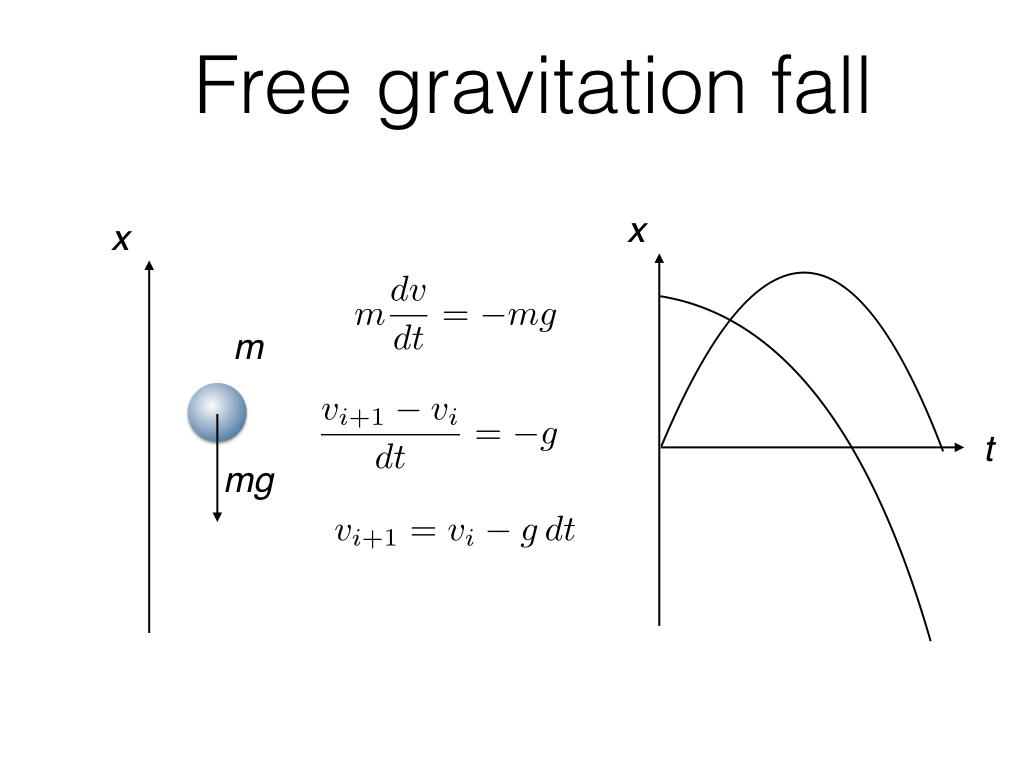
\includegraphics{../figs/ode.002.jpeg}
\caption{simple\_gravitation\_fall}
\end{figure}

    \subsection{Euler法}\label{eulerux6cd5}

1次の微分方程式の一般形は

\[
\frac{dx}{dt}=f(x,t)
\]
と書けます.この微分方程式を簡単な近似から求めるオイラー法を示します.
\(x(t+\delta t)\)をテイラー級数展開すると,

\[
x(t+\delta t) \simeq x(t) + \frac{dx}{dt} \delta t
\]
となります.これらを代入すると,計算アルゴリズムはつぎのようになります,

\[
x_{i+1} = x_i + f_i\,\delta t
\]
ここで,\(f_i\)は点(\(x_i, t_i\))における関数の値です.このアルゴリズムを適用して,\(t+\delta t\)の座標\(x_{i+1}\)を一つ前の時間の座標\(x_i\)から導くことができます.これを重力場中の運動方程式に適用します.

    \subsection{重力場中の運動をEuler法で解いたら}\label{ux91cdux529bux5834ux4e2dux306eux904bux52d5ux3092eulerux6cd5ux3067ux89e3ux3044ux305fux3089}

Euler法は一階の微分方程式に対する定式化をしています.ところが,重力場中の運動は2階の微分方程式です.このようなときには媒介変数を導入して1次連立方程式に置き直します.

媒介変数として速度\(v\)を使って,2階の運動方程式 \[
\frac{d^2x}{dt^2} = -g 
\] が,1階の連立方程式 \[
\begin{aligned}
\frac{dv}{dt} & = -g \\
\frac{dx}{dt} & = v 
\end{aligned}
\] で置き換えられると考えることに相当します.アルゴリズムにすると,

\[
\begin{aligned}
v_{i+1} &= v_i - g\, dt \\
x_{i+1} &= x_i + v_i\, dt
\end{aligned}
\]
なる連立方程式を解くことに置き換わります.これをMapleで関数にして,さらに計算結果を表示させてみます.

    \begin{Verbatim}[commandchars=\\\{\}]
{\color{incolor}In [{\color{incolor} }]:} \PY{n+no}{Euler} \PY{p}{:}\PY{o}{=} \PY{n+nb}{proc} \PY{p}{(}\PY{n}{x\PYZus{}i}\PY{p}{,} \PY{n}{v\PYZus{}i}\PY{p}{)}
          \PY{n}{local} \PY{n}{v\PYZus{}ip1}\PY{p}{,} \PY{n}{x\PYZus{}ip1}\PY{p}{;}
          \PY{n}{global} \PY{n}{g}\PY{p}{,} \PY{n}{dt}\PY{p}{;}
          \PY{n}{v\PYZus{}ip1} \PY{p}{:}\PY{o}{=} \PY{n}{v\PYZus{}i} \PY{o}{\PYZhy{}} \PY{n}{g} \PY{o}{*} \PY{n}{dt}\PY{p}{;}
          \PY{n}{x\PYZus{}ip1} \PY{p}{:}\PY{o}{=} \PY{n}{x\PYZus{}i} \PY{o}{+} \PY{n}{v\PYZus{}i} \PY{o}{*} \PY{n}{dt}\PY{p}{;}
          \PY{k}{return} \PY{n}{x\PYZus{}ip1}\PY{p}{,} \PY{n}{v\PYZus{}ip1}\PY{p}{;}
        \PY{k}{end}\PY{p}{;}
\end{Verbatim}


    Eulerはx\_i, v\_iを受け取って,先ほど導いた簡単な計算によって,v\_i+1,
x\_i+1を順次計算して返します.結果は,

    \begin{Verbatim}[commandchars=\\\{\}]
{\color{incolor}In [{\color{incolor} }]:} \PY{l+s+ss}{dt}\PY{p}{:}\PY{o}{=}\PY{l+m+mi}{0}\PY{o}{.}\PY{l+m+mi}{1}\PY{p}{;}\PY{l+s+ss}{g}\PY{p}{:}\PY{o}{=}\PY{l+m+mi}{0}\PY{o}{.}\PY{l+m+mi}{1}\PY{p}{;} 
        \PY{l+s+ss}{vv}\PY{p}{:}\PY{o}{=}\PY{o}{[}\PY{l+m+mi}{0}\PY{o}{]}\PY{p}{;}
        \PY{l+s+ss}{xx}\PY{p}{:}\PY{o}{=}\PY{o}{[}\PY{l+m+mi}{10}\PY{o}{]}\PY{p}{;}
        
        \PY{k}{for} \PY{n}{i} \PY{n}{from} \PY{l+m+mi}{2} \PY{n}{to} \PY{l+m+mi}{200} \PY{k}{do}
          \PY{n}{x}\PY{p}{,} \PY{n}{v} \PY{p}{:}\PY{o}{=} \PY{n+no}{Euler}\PY{p}{(}\PY{n}{xx}\PY{o}{[}\PY{n}{i}\PY{o}{\PYZhy{}}\PY{l+m+mi}{1}\PY{o}{]}\PY{p}{,}\PY{n}{vv}\PY{o}{[}\PY{n}{i}\PY{o}{\PYZhy{}}\PY{l+m+mi}{1}\PY{o}{]}\PY{p}{)}\PY{p}{;}
          \PY{n}{xx} \PY{p}{:}\PY{o}{=}\PY{o}{[}\PY{n}{op}\PY{p}{(}\PY{n}{xx}\PY{p}{)}\PY{p}{,}\PY{n}{x}\PY{o}{]}\PY{p}{;} 
          \PY{n}{vv} \PY{p}{:}\PY{o}{=}\PY{o}{[}\PY{n}{op}\PY{p}{(}\PY{n}{vv}\PY{p}{)}\PY{p}{,}\PY{n}{v}\PY{o}{]}\PY{p}{;} 
        \PY{k}{end} \PY{k}{do}\PY{p}{:}
        
        \PY{n}{with}\PY{p}{(}\PY{n}{plots}\PY{p}{)}\PY{p}{:}
        \PY{n}{listplot}\PY{p}{(}\PY{n}{xx}\PY{p}{)}\PY{p}{;}
        \PY{n}{listplot}\PY{p}{(}\PY{n}{vv}\PY{p}{)}\PY{p}{;}
\end{Verbatim}


    位置(\(x\))と速度(\(v\))の時間(\(t\))変化を表示させています.

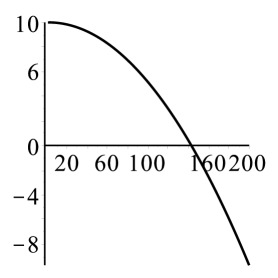
\includegraphics{../figs/Euler_ball_dropplot2d1.jpg}
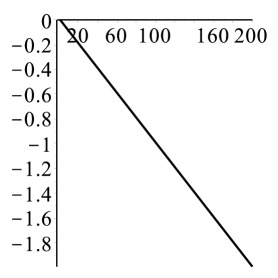
\includegraphics{../figs/Euler_ball_dropplot2d2.jpg}

時間とともに位置は放物線状に変化し,速度は一定の傾きで増加していく,等加速度運動を再現しています.Euler法ではこのように非常に簡単なcodeによって微分方程式で表される現象をシミュレートできることがわかるでしょう.

    \subsection{空気抵抗がある水滴の落下}\label{ux7a7aux6c17ux62b5ux6297ux304cux3042ux308bux6c34ux6ef4ux306eux843dux4e0b}

ballの落下ではわかりにくいですが,より小さな質量の水滴では,速度に比例する空気抵抗が効いてきます.この様子を見ましょう.微分方程式には,

\[
F_x = - C v_x
\]

項が付与されます.そうすると運動方程式は

\[
m \frac{dv_x}{dt} = - C v_x - mg
\]
となります.これにともなったv\_xの時間変化に対して,今までは単純に重力加速していたのが,v\_xに比例する空気抵抗を記述する項が付与されます.この変化をEuler2に入れ込むと少しの修正ですが,結果は劇的に変化します.

\begin{figure}[htbp]
\centering
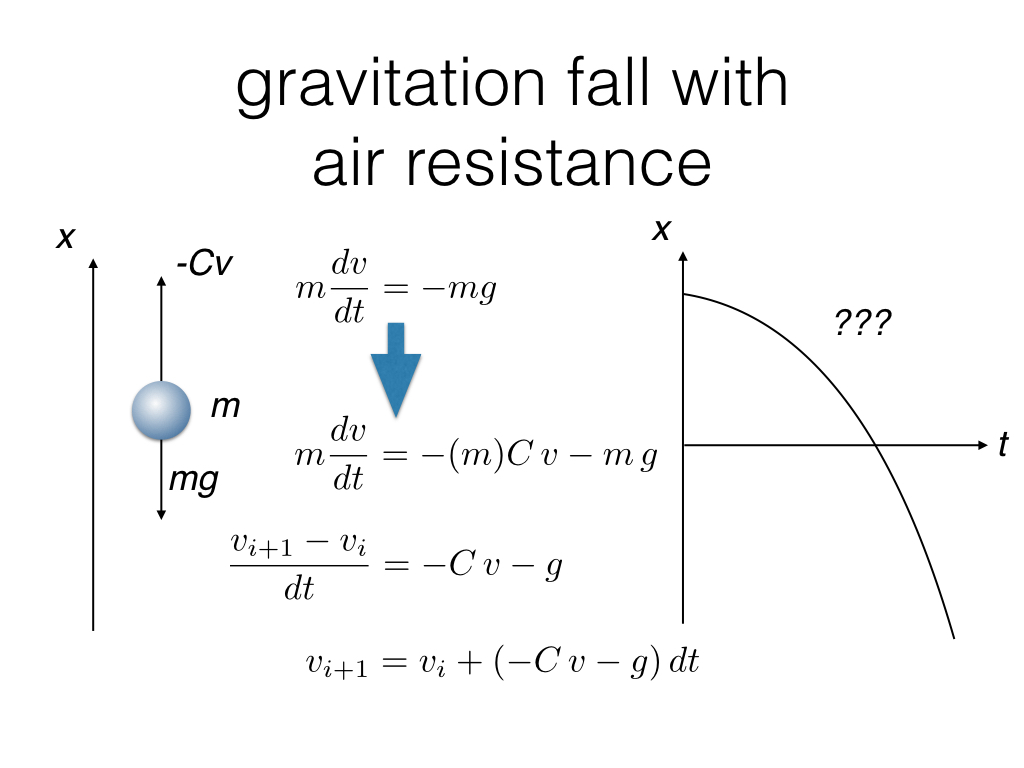
\includegraphics{../figs/ode.003.jpeg}
\caption{gravitation\_fall\_with\_air\_resistance}
\end{figure}

    \begin{Verbatim}[commandchars=\\\{\}]
{\color{incolor}In [{\color{incolor} }]:} \PY{n+no}{Euler2} \PY{p}{:}\PY{o}{=} \PY{n+nb}{proc} \PY{p}{(}\PY{n}{x\PYZus{}i}\PY{p}{,} \PY{n}{v\PYZus{}i}\PY{p}{)}
          \PY{n}{local} \PY{n}{v\PYZus{}ip1}\PY{p}{,} \PY{n}{x\PYZus{}ip1}\PY{p}{;}
          \PY{n}{global} \PY{n}{g}\PY{p}{,} \PY{n}{dt}\PY{p}{;}
          \PY{n}{v\PYZus{}ip1} \PY{p}{:}\PY{o}{=} \PY{n}{v\PYZus{}i} \PY{o}{+} \PY{p}{(}\PY{o}{\PYZhy{}}\PY{n}{cc} \PY{o}{*} \PY{n}{v\PYZus{}i}\PY{o}{\PYZhy{}} \PY{n}{g}\PY{p}{)} \PY{o}{*} \PY{n}{dt}\PY{p}{;}
          \PY{n}{x\PYZus{}ip1} \PY{p}{:}\PY{o}{=} \PY{n}{x\PYZus{}i} \PY{o}{+} \PY{n}{v\PYZus{}i} \PY{o}{*} \PY{n}{dt}\PY{p}{;}
          \PY{k}{return} \PY{n}{x\PYZus{}ip1}\PY{p}{,} \PY{n}{v\PYZus{}ip1}\PY{p}{;}
        \PY{k}{end}\PY{p}{:}
        
        \PY{l+s+ss}{dt}\PY{p}{:}\PY{o}{=}\PY{l+m+mi}{0}\PY{o}{.}\PY{l+m+mi}{1}\PY{p}{:} \PY{l+s+ss}{g}\PY{p}{:}\PY{o}{=}\PY{l+m+mi}{0}\PY{o}{.}\PY{l+m+mi}{1}\PY{p}{:} \PY{l+s+ss}{cc}\PY{p}{:}\PY{o}{=}\PY{l+m+mi}{1}\PY{p}{:}
\end{Verbatim}


    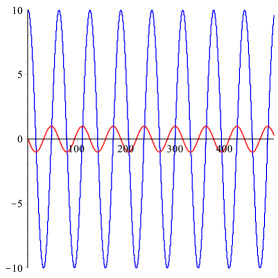
\includegraphics{../figs/Euler_ball_dropplot2d4.jpg}
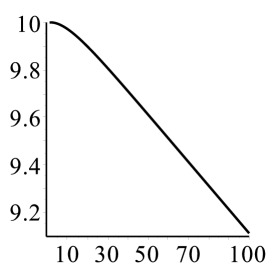
\includegraphics{../figs/Euler_ball_dropplot2d3.jpg}

速度は空気抵抗によって,一定となります.またそれに伴って位置は一定の傾きで落ちていきます.空気抵抗がないときに加速が続く様子とは違った挙動が観察できるでしょう.電車の窓に落ちる雨粒がまっすぐつくのはそのせいです.たぶん...

    \section{高精度計算}\label{ux9ad8ux7cbeux5ea6ux8a08ux7b97}

\subsection{バネの運動}\label{ux30d0ux30cdux306eux904bux52d5}

今度はバネの運動です.空気抵抗との違いはほんの少しで, \[
F_x = -k x
\] と今度は,位置xに力が比例することです.そうすると運動方程式は,

\[
m \frac{dv_x}{dt} = - k x
\] となります.

連立方程式は \[
\begin{aligned}
\frac{dv}{dt} & = - \frac{k}{m}x \\
\frac{dx}{dt} & = v
\end{aligned}
\] となるんで,アルゴリズムに置き換えると,

\[
\begin{aligned}
v_{i+1} & = v_i - \frac{k}{m} x_i\, dt \\
x_{i+1} & = x_i + v_i\, dt
\end{aligned}
\]
なる連立方程式を解くことに置き換わります.これをMapleで関数にして,さらに計算結果を表示させてみます.

\begin{figure}[htbp]
\centering
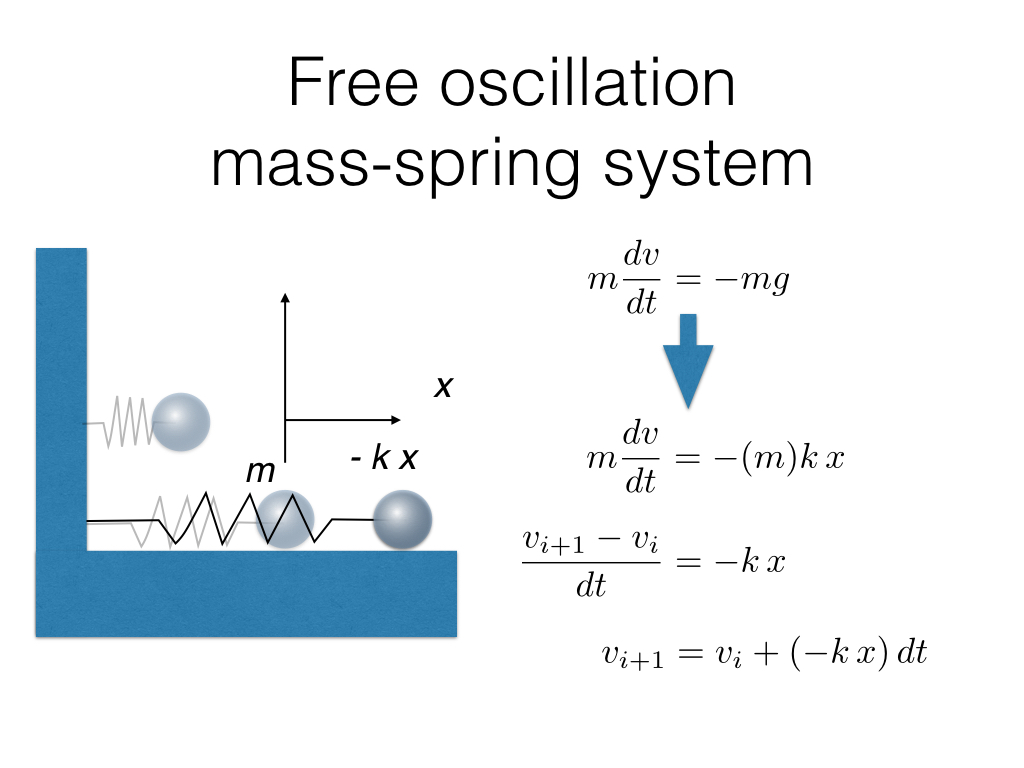
\includegraphics{../figs/ode.004.jpeg}
\caption{free\_oscillation\_mass\_sprint\_system}
\end{figure}

    \begin{Verbatim}[commandchars=\\\{\}]
{\color{incolor}In [{\color{incolor} }]:} \PY{n+no}{Euler3} \PY{p}{:}\PY{o}{=} \PY{n+nb}{proc} \PY{p}{(}\PY{n}{x\PYZus{}0}\PY{p}{,} \PY{n}{v\PYZus{}0}\PY{p}{)}
          \PY{n}{local} \PY{n}{v\PYZus{}1}\PY{p}{,} \PY{n}{x\PYZus{}1}\PY{p}{;}
          \PY{n}{global} \PY{n}{k}\PY{p}{,} \PY{n}{cc}\PY{p}{,} \PY{n}{dx}\PY{p}{;}
          \PY{n}{v\PYZus{}1} \PY{p}{:}\PY{o}{=} \PY{n}{v\PYZus{}0} \PY{o}{+} \PY{p}{(}\PY{o}{\PYZhy{}} \PY{n}{k} \PY{o}{*} \PY{n}{x\PYZus{}0}\PY{p}{)} \PY{o}{*} \PY{n}{dt}\PY{p}{;}
          \PY{n}{x\PYZus{}1} \PY{p}{:}\PY{o}{=} \PY{n}{x\PYZus{}0} \PY{o}{+} \PY{n}{v\PYZus{}0} \PY{o}{*} \PY{n}{dt}\PY{p}{;}
          \PY{k}{return} \PY{n}{x\PYZus{}1}\PY{p}{,} \PY{n}{v\PYZus{}1}\PY{p}{;}
        \PY{k}{end}\PY{p}{;}
        
        \PY{l+s+ss}{dt}\PY{p}{:}\PY{o}{=}\PY{l+m+mi}{0}\PY{o}{.}\PY{l+m+mi}{1}\PY{p}{;}\PY{l+s+ss}{k}\PY{p}{:}\PY{o}{=}\PY{l+m+mi}{0}\PY{o}{.}\PY{l+m+mo}{01}\PY{p}{;}
        \PY{l+s+ss}{vv}\PY{p}{:}\PY{o}{=}\PY{o}{[}\PY{l+m+mi}{0}\PY{o}{.}\PY{l+m+mo}{01}\PY{o}{]}\PY{p}{;}
        \PY{l+s+ss}{xx}\PY{p}{:}\PY{o}{=}\PY{o}{[}\PY{l+m+mi}{0}\PY{o}{]}\PY{p}{;} 
        \PY{k}{for} \PY{n}{i} \PY{n}{from} \PY{l+m+mi}{2} \PY{n}{to} \PY{l+m+mi}{4000} \PY{k}{do}
          \PY{n}{x}\PY{p}{,} \PY{n}{v} \PY{p}{:}\PY{o}{=} \PY{n+no}{Euler3}\PY{p}{(}\PY{n}{xx}\PY{o}{[}\PY{n}{i}\PY{o}{\PYZhy{}}\PY{l+m+mi}{1}\PY{o}{]}\PY{p}{,}\PY{n}{vv}\PY{o}{[}\PY{n}{i}\PY{o}{\PYZhy{}}\PY{l+m+mi}{1}\PY{o}{]}\PY{p}{)}\PY{p}{;}
          \PY{n}{xx} \PY{p}{:}\PY{o}{=}\PY{o}{[}\PY{n}{op}\PY{p}{(}\PY{n}{xx}\PY{p}{)}\PY{p}{,}\PY{n}{x}\PY{o}{]}\PY{p}{;} 
          \PY{n}{vv} \PY{p}{:}\PY{o}{=}\PY{o}{[}\PY{n}{op}\PY{p}{(}\PY{n}{vv}\PY{p}{)}\PY{p}{,}\PY{n}{v}\PY{o}{]}\PY{p}{;} 
        \PY{k}{end} \PY{k}{do}\PY{p}{:}
        \PY{n}{with}\PY{p}{(}\PY{n}{plots}\PY{p}{)}\PY{p}{:}
        \PY{n}{listplot}\PY{p}{(}\PY{n}{xx}\PY{p}{)}\PY{p}{;}\PY{n}{listplot}\PY{p}{(}\PY{n}{vv}\PY{p}{)}\PY{p}{;}
\end{Verbatim}


    kはあらかじめ\(m\)で割られて正規化されているとします.これをEuler法で計算すると次のような結果が得られます.

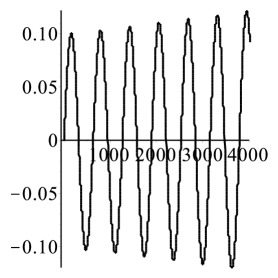
\includegraphics{../figs/springplot2d1.jpg}
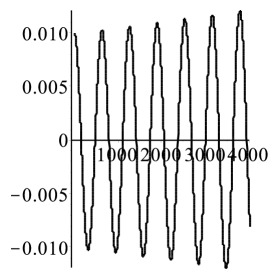
\includegraphics{../figs/springplot2d2.jpg}

徐々に発散していく様子がわかると思います.本来,摩擦のないバネは定常的に振動します.この発散の原因は,Euler法の計算誤差が大きいせいです.そこで,より精度の高いRunge-Kutta法を導入します.

    \subsection{2次のRunge-Kuttaの導出}\label{ux6b21ux306erunge-kuttaux306eux5c0eux51fa}

一般にRunge-Kutta法と呼ばれる手法は,4次の古典的Runge-Kutta法を指します.導出は意外と面倒なので,2次の場合のさわりを紹介して,そこからの類推としましょう.\(x,v,t\)などのパラメータ名を変更しますのでご注意あれ.

(「ANSI Cによる数値計算法」堀之内聰一,酒井幸吉,榎園茂,森北2002,
p.133) テイラー展開により,\(h^2\)の精度まで展開する. \[
y(x_0+h) = y(x_0) +y_0'h+\frac{1}{2!}y_0''h^2 + O(h^3)
\]

この式において,\(y_0' = f(x_0,y_0)\)は既知とする.一方,\(y_0''\)は\(f(x_0,y_0)\)から直接的には求められない.したがって,この式の右辺と\(h^2\)の項まで一致する近似値を,\(f(x_0,y_0)\)だけを既知として算出する方法を考えよう.

平均値の定理より, \[
\Delta y = y(x_0+h)-y(x_0) = hy'(x_0 + \theta h), \, 0<\theta<1
\]

\(y'(x_0 +\theta h)\)の近似値として,\(\theta=0, \theta=1\)の場合を考えると,
\[
\begin{aligned}
\Delta y &\simeq hy'(x_0) \, &{\textrm where}\, &\theta=0\\
\Delta y &\simeq hy'(x_0+h)  \, &{\textrm where}\, &\theta=1
\end{aligned}
\]
これらの値は単独では\(\Delta y\)に対して\(h^2\)の精度をもつ近似値にならないが,これらの一次結合\(\alpha h y'(x_0)+\beta hy'(x_0+h)\)を\(\alpha, \beta\)をうまく定めることによって,\(\Delta y\)の\(h^2\)の精度をもつ近似値にすることができる.実際,
\[
\begin{aligned}
\alpha h y'(x_0)+\beta hy'(x_0+h) & =\alpha h y'(x_0)+\beta h \{y'(x+0)+y''(x_0)h+O(h^2)\} \\
& =(\alpha+\beta)hy'_0 + \beta h^2 y_0'' + O(h^3)
\end{aligned}
\]

したがって,テイラー展開式と係数を比較して, \[
\begin{aligned}
\alpha + \beta = 1, \, \beta = \frac{1}{2}\\
\alpha = \frac{1}{2}, \, \beta =\frac{1}{2}
\end{aligned}\] となり,

\[
\Delta y = \frac{1}{2}hy'(x_0) + \frac{1}{2}hy'(x_0+h)+O(h^3)
\]

いま, \[
k_1 =hy'(x_0) =hf(x_0,y_0)
\]

とおこう.上式に代入して, \[
\begin{aligned}
hy'(x_0+h) &= hf(x_0+h,y(x_0+h)) \\
& =hf(x_0+h, y(x_0)+y'(x_o)h+O(h^2)) \\
& =hf(x_0+h, y_0+k_1+O(h^2)) \\
& =hf(x_0+h, y_0+k_1)+O(h^2)
\end{aligned}\]

したがって, \[
k_2 = hf(x_0+h, y_0+k_1)
\] とおけば, \[
\Delta y = \frac{1}{2}k_1 + \frac{1}{2}k_2 + O(h^3)
\] となる.これより, \[
k = \frac{1}{2}(k_1+k_2), y_1 = y_0 +k
\]

とおくと,\(y(x_0+h) = y_1+O(h^3)\)となり,\(y_1\)は\(h^2\)の精度の近似値となる.

    \subsection{Runge-Kutta2次公式}\label{runge-kutta2ux6b21ux516cux5f0f}

こうして得られたRunge-Kuttaの2次の公式を定義すると次の通りです.

微分方程式 \[
\frac{dy}{dx} = f(x,y), \, where \, y(x_0)=y_0
\]

の数値解は,刻み幅を\(h\),\(x_n=x_0+nh\)として,次の漸化式 \[
y_{n+1} = y_n +k (n=0,1,2,\cdots)
\] で与えられる.ここに,\(k\)は次で定める. \[
\begin{aligned}
k_1 & = hf(x_n,y_n), \\
k_2 & = hf(x_n+h, y_n+k_1), \\
k & = \frac{1}{2}(k_1+k_2)
\end{aligned}
\]

    \subsection{Runge-Kutta4次公式}\label{runge-kutta4ux6b21ux516cux5f0f}

2次と同様の考え方で,\(h^4\)の精度を持つRunge-Kutta4次公式を作ることができる.

微分方程式 \[
\frac{dy}{dx} = f(x,y), \, {\textrm where}y(x_0)=y_0
\]

の数値解は,刻み幅を\(h\),\(x_n=x_0+nh\)として,次の漸化式 \[
y_{n+1} = y_n +k (n=0,1,2,\cdots)
\] で与えられる.ここに,\(k\)は次で定める. \[
\begin{aligned}
k_1 & = hf(x_n,y_n), \\
k_2 & = hf(x_n+\frac{h}{2}, y_n+\frac{k_1}{2}), \\
k_3 & = hf(x_n+\frac{h}{2}, y_n+\frac{k_2}{2}), \\
k_4 & = hf(x_n+h, y_n+k_3), \\
k & = \frac{1}{6}(k_1+2k_2+2k_3+k_4)
\end{aligned}
\]

    \subsection{連立方程式にRunge-Kutta4次公式を}\label{ux9023ux7acbux65b9ux7a0bux5f0fux306brunge-kutta4ux6b21ux516cux5f0fux3092}

連立微分方程式 \[
\begin{aligned}
\frac{dy}{dx} &= f(x,y,z), &\, \, where \, y(x_0)=y_0 \\
\frac{dz}{dx} &= g(x,y,z), &\, \, where \, z(x_0)=z_0 \\
\end{aligned}
\]

の数値解は,刻み幅を\(h\),\(x_n=x_0+nh\)として,次の漸化式 \[
\begin{aligned}
y_{n+1} & = y_n +k &\, (n=0,1,2,\cdots) \\
z_{n+1} & = z_n +l &\, (n=0,1,2,\cdots) \\
\end{aligned}
\] で与えられる.ここに,\(k,l\)は次で定める. \[
\begin{aligned}
k_1 &= hf(x_n,y_n,z_n), \,
&l_1 &= hg(x_n,y_n,z_n), \\
k_2 &= hf(x_n+\frac{h}{2}, y_n+\frac{k_1}{2}, z_n+\frac{l_1}{2}), \,
&l_2 &= hg(x_n+\frac{h}{2}, y_n+\frac{k_1}{2}, z_n+\frac{l_1}{2}), \\
k_3 &= hf(x_n+\frac{h}{2}, y_n+\frac{k_2}{2}, z_n+\frac{l_2}{2}), \,
&l_3 &= hg(x_n+\frac{h}{2}, y_n+\frac{k_2}{2}, z_n+\frac{l_2}{2}), \\
k_4 &= hf(x_n+h, y_n+k_3, z_n+l_3), \,
&l_4 &= hg(x_n+h, y_n+k_3, z_n+l_3), \\
k &= \frac{1}{6}(k_1+2k_2+2k_3+k_4), \,
&l &= \frac{1}{6}(l_1+2l_2+2l_3+l_4)
\end{aligned}
\]

    \begin{Verbatim}[commandchars=\\\{\}]
{\color{incolor}In [{\color{incolor} }]:} \PY{n+no}{RungeKutta4} \PY{p}{:}\PY{o}{=} \PY{n+nb}{proc}\PY{p}{(}\PY{n}{x\PYZus{}i}\PY{p}{,}\PY{n}{y\PYZus{}i}\PY{p}{,}\PY{n}{z\PYZus{}i}\PY{p}{,}\PY{n}{h}\PY{p}{)}
          \PY{n}{local} \PY{n}{k1}\PY{p}{,}\PY{n}{l1}\PY{p}{,}\PY{n}{k2}\PY{p}{,}\PY{n}{l2}\PY{p}{,}\PY{n}{k3}\PY{p}{,}\PY{n}{l3}\PY{p}{,}\PY{n}{k4}\PY{p}{,}\PY{n}{l4}\PY{p}{,}\PY{n}{kk}\PY{p}{,}\PY{n}{ll}\PY{p}{;}
          \PY{l+s+ss}{k1}\PY{p}{:}\PY{o}{=} \PY{n}{h} \PY{o}{*} \PY{n}{ff}\PY{p}{(}\PY{n}{x\PYZus{}i}\PY{p}{,} \PY{n}{y\PYZus{}i}\PY{p}{,} \PY{n}{z\PYZus{}i}\PY{p}{)}\PY{p}{;}
          \PY{l+s+ss}{l1}\PY{p}{:}\PY{o}{=} \PY{n}{h} \PY{o}{*} \PY{n}{gg}\PY{p}{(}\PY{n}{x\PYZus{}i}\PY{p}{,} \PY{n}{y\PYZus{}i}\PY{p}{,} \PY{n}{z\PYZus{}i}\PY{p}{)}\PY{p}{;}
          \PY{l+s+ss}{k2}\PY{p}{:}\PY{o}{=} \PY{n}{h} \PY{o}{*} \PY{n}{ff}\PY{p}{(}\PY{n}{x\PYZus{}i} \PY{o}{+} \PY{n}{h}\PY{o}{/}\PY{l+m+mi}{2}\PY{p}{,} \PY{n}{y\PYZus{}i} \PY{o}{+} \PY{n}{k1}\PY{o}{/}\PY{l+m+mi}{2}\PY{p}{,} \PY{n}{z\PYZus{}i} \PY{o}{+} \PY{n}{l1}\PY{o}{/}\PY{l+m+mi}{2}\PY{p}{)}\PY{p}{;}
          \PY{l+s+ss}{l2}\PY{p}{:}\PY{o}{=} \PY{n}{h} \PY{o}{*} \PY{n}{gg}\PY{p}{(}\PY{n}{x\PYZus{}i} \PY{o}{+} \PY{n}{h}\PY{o}{/}\PY{l+m+mi}{2}\PY{p}{,} \PY{n}{y\PYZus{}i} \PY{o}{+} \PY{n}{k1}\PY{o}{/}\PY{l+m+mi}{2}\PY{p}{,} \PY{n}{z\PYZus{}i} \PY{o}{+} \PY{n}{l1}\PY{o}{/}\PY{l+m+mi}{2}\PY{p}{)}\PY{p}{;}
          \PY{l+s+ss}{k3}\PY{p}{:}\PY{o}{=} \PY{n}{h} \PY{o}{*} \PY{n}{ff}\PY{p}{(}\PY{n}{x\PYZus{}i} \PY{o}{+} \PY{n}{h}\PY{o}{/}\PY{l+m+mi}{2}\PY{p}{,} \PY{n}{y\PYZus{}i} \PY{o}{+} \PY{n}{k2}\PY{o}{/}\PY{l+m+mi}{2}\PY{p}{,} \PY{n}{z\PYZus{}i} \PY{o}{+} \PY{n}{l2}\PY{o}{/}\PY{l+m+mi}{2}\PY{p}{)}\PY{p}{;}
          \PY{l+s+ss}{l3}\PY{p}{:}\PY{o}{=} \PY{n}{h} \PY{o}{*} \PY{n}{gg}\PY{p}{(}\PY{n}{x\PYZus{}i} \PY{o}{+} \PY{n}{h}\PY{o}{/}\PY{l+m+mi}{2}\PY{p}{,} \PY{n}{y\PYZus{}i} \PY{o}{+} \PY{n}{k2}\PY{o}{/}\PY{l+m+mi}{2}\PY{p}{,} \PY{n}{z\PYZus{}i} \PY{o}{+} \PY{n}{l2}\PY{o}{/}\PY{l+m+mi}{2}\PY{p}{)}\PY{p}{;}
          \PY{l+s+ss}{k4}\PY{p}{:}\PY{o}{=} \PY{n}{h} \PY{o}{*} \PY{n}{ff}\PY{p}{(}\PY{n}{x\PYZus{}i} \PY{o}{+} \PY{n}{h}\PY{p}{,}   \PY{n}{y\PYZus{}i} \PY{o}{+} \PY{n}{k3}\PY{p}{,}   \PY{n}{z\PYZus{}i} \PY{o}{+} \PY{n}{l3}\PY{p}{)}\PY{p}{;}
          \PY{l+s+ss}{l4}\PY{p}{:}\PY{o}{=} \PY{n}{h} \PY{o}{*} \PY{n}{gg}\PY{p}{(}\PY{n}{x\PYZus{}i} \PY{o}{+} \PY{n}{h}\PY{p}{,}   \PY{n}{y\PYZus{}i} \PY{o}{+} \PY{n}{k3}\PY{p}{,}   \PY{n}{z\PYZus{}i} \PY{o}{+} \PY{n}{l3}\PY{p}{)}\PY{p}{;}
          \PY{n}{kk} \PY{p}{:}\PY{o}{=} \PY{l+m+mi}{1}\PY{o}{/}\PY{l+m+mi}{6}\PY{o}{*}\PY{p}{(}\PY{n}{k1} \PY{o}{+} \PY{l+m+mi}{2}\PY{o}{*}\PY{n}{k2} \PY{o}{+} \PY{l+m+mi}{2}\PY{o}{*}\PY{n}{k3} \PY{o}{+} \PY{n}{k4}\PY{p}{)}\PY{p}{;}
          \PY{n}{ll} \PY{p}{:}\PY{o}{=} \PY{l+m+mi}{1}\PY{o}{/}\PY{l+m+mi}{6}\PY{o}{*}\PY{p}{(}\PY{n}{l1} \PY{o}{+} \PY{l+m+mi}{2}\PY{o}{*}\PY{n}{l2} \PY{o}{+} \PY{l+m+mi}{2}\PY{o}{*}\PY{n}{l3} \PY{o}{+} \PY{n}{l4}\PY{p}{)}\PY{p}{;}
          \PY{k}{return} \PY{n}{kk}\PY{p}{,}\PY{n}{ll}\PY{p}{;}
        \PY{k}{end}\PY{p}{:}
\end{Verbatim}


    Runge-Kuttaの4次公式をそのままcodingすると上のようになります.これを先ほどのバネ運動の問題に当てはめてみましょう.

先ほど導出した運動方程式の漸化式 \[
\begin{aligned}
v_{i+1} & = v_i - \frac{k}{m} x_i\, dt \\
x_{i+1} & = x_i + v_i\, dt
\end{aligned}
\]

とRunge-Kutta4次公式を示した連立微分方程式 \[
\begin{aligned}
\frac{dy}{dx} &= f(x,y,z), \, where \, y(x_0)=y_0 \\
\frac{dz}{dx} &= g(x,y,z), \, where \, z(x_0)=z_0 \\
\end{aligned}
\] とを比べて,変数の表記の違いと関数\(f,g\)を具体的に書き下します.

\begin{longtable}[]{@{}cc@{}}
\toprule
4次の公式 & 運動方程式\tabularnewline
\midrule
\endhead
x & t\tabularnewline
y & x\tabularnewline
z & v\tabularnewline
f(x,y,z) & f(t,x,v) = v\tabularnewline
g(x,y,z) & g(t,x,v) = -k x\tabularnewline
\bottomrule
\end{longtable}

この変数の書き換えを吸収する中間関数としてEuler3を書き換えます.RungeKutta4の仮引数を上の表に従って置き換えて,数値を渡しています.また,関数\(f,g\)も定義しておきます.

    \begin{Verbatim}[commandchars=\\\{\}]
{\color{incolor}In [{\color{incolor} }]:} \PY{n}{ff} \PY{p}{:}\PY{o}{=} \PY{p}{(}\PY{n}{t}\PY{p}{,}\PY{n}{x}\PY{p}{,}\PY{n}{v}\PY{p}{)}\PY{o}{\PYZhy{}}\PY{o}{\PYZgt{}} \PY{n}{v}\PY{p}{;}
        \PY{n}{gg} \PY{p}{:}\PY{o}{=} \PY{p}{(}\PY{n}{t}\PY{p}{,}\PY{n}{x}\PY{p}{,}\PY{n}{v}\PY{p}{)}\PY{o}{\PYZhy{}}\PY{o}{\PYZgt{}} \PY{o}{\PYZhy{}}\PY{n}{k}\PY{o}{*}\PY{n}{x}\PY{p}{;}
        
        \PY{n+no}{Euler3} \PY{p}{:}\PY{o}{=} \PY{n+nb}{proc} \PY{p}{(}\PY{n}{x\PYZus{}0}\PY{p}{,} \PY{n}{v\PYZus{}0}\PY{p}{)}
          \PY{n}{local} \PY{n}{v\PYZus{}1}\PY{p}{,} \PY{n}{x\PYZus{}1}\PY{p}{,} \PY{n}{kk}\PY{p}{,} \PY{n}{ll}\PY{p}{;}
          \PY{n}{global} \PY{n}{dt}\PY{p}{;}
          \PY{n}{kk}\PY{p}{,}\PY{n}{ll} \PY{p}{:}\PY{o}{=} \PY{n+no}{RungeKutta4}\PY{p}{(}\PY{n}{t}\PY{p}{,} \PY{n}{x\PYZus{}0}\PY{p}{,} \PY{n}{v\PYZus{}0}\PY{p}{,} \PY{n}{dt}\PY{p}{)}\PY{p}{;}
          \PY{l+s+ss}{x\PYZus{}1}\PY{p}{:}\PY{o}{=} \PY{n}{x\PYZus{}0} \PY{o}{+} \PY{n}{kk}\PY{p}{;}
          \PY{l+s+ss}{v\PYZus{}1}\PY{p}{:}\PY{o}{=} \PY{n}{v\PYZus{}0} \PY{o}{+} \PY{n}{ll}\PY{p}{;}
          \PY{k}{return} \PY{n}{x\PYZus{}1}\PY{p}{,} \PY{n}{v\PYZus{}1}\PY{p}{;}
        \PY{k}{end}\PY{p}{;}
\end{Verbatim}


    \begin{Verbatim}[commandchars=\\\{\}]
{\color{incolor}In [{\color{incolor} }]:} \PY{l+s+ss}{dt}\PY{p}{:}\PY{o}{=}\PY{l+m+mi}{0}\PY{o}{.}\PY{l+m+mi}{1}\PY{p}{;}\PY{l+s+ss}{k}\PY{p}{:}\PY{o}{=}\PY{l+m+mi}{0}\PY{o}{.}\PY{l+m+mo}{01}\PY{p}{;}
        \PY{l+s+ss}{vv}\PY{p}{:}\PY{o}{=}\PY{o}{[}\PY{l+m+mi}{0}\PY{o}{.}\PY{l+m+mo}{01}\PY{o}{]}\PY{p}{;}
        \PY{l+s+ss}{xx}\PY{p}{:}\PY{o}{=}\PY{o}{[}\PY{l+m+mi}{0}\PY{o}{]}\PY{p}{;} 
        \PY{k}{for} \PY{n}{i} \PY{n}{from} \PY{l+m+mi}{2} \PY{n}{to} \PY{l+m+mi}{4000} \PY{k}{do}
          \PY{n}{x}\PY{p}{,} \PY{n}{y} \PY{p}{:}\PY{o}{=} \PY{n+no}{Euler3}\PY{p}{(}\PY{n}{xx}\PY{o}{[}\PY{n}{i}\PY{o}{\PYZhy{}}\PY{l+m+mi}{1}\PY{o}{]}\PY{p}{,}\PY{n}{vv}\PY{o}{[}\PY{n}{i}\PY{o}{\PYZhy{}}\PY{l+m+mi}{1}\PY{o}{]}\PY{p}{)}\PY{p}{;}
          \PY{n}{xx} \PY{p}{:}\PY{o}{=}\PY{o}{[}\PY{n}{op}\PY{p}{(}\PY{n}{xx}\PY{p}{)}\PY{p}{,}\PY{n}{x}\PY{o}{]}\PY{p}{;} 
          \PY{n}{vv} \PY{p}{:}\PY{o}{=}\PY{o}{[}\PY{n}{op}\PY{p}{(}\PY{n}{vv}\PY{p}{)}\PY{p}{,}\PY{n}{y}\PY{o}{]}\PY{p}{;} 
        \PY{k}{end} \PY{k}{do}\PY{p}{:}
        \PY{n}{with}\PY{p}{(}\PY{n}{plots}\PY{p}{)}\PY{p}{:}
        \PY{n}{listplot}\PY{p}{(}\PY{n}{xx}\PY{p}{)}\PY{p}{;}\PY{n}{listplot}\PY{p}{(}\PY{n}{vv}\PY{p}{)}\PY{p}{;}
\end{Verbatim}


    これを前と同様に走らせると

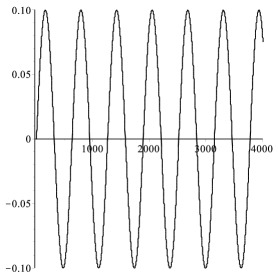
\includegraphics{../figs/springplot2d3.jpg}
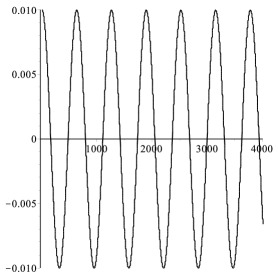
\includegraphics{../figs/springplot2d4.jpg}

発散も収束もすることなく,定常的に振動を繰り返していることが見て取れます.

    \section{電気回路の応答}\label{ux96fbux6c17ux56deux8defux306eux5fdcux7b54}

電気回路の応答を考えましょう.LRCをふたつずつ組み合わせてみていくのが常套手段なんですが,一個ずつだと面倒なので,まずは全部入れた方程式を立てます.そこからパラメータを変えて回路の挙動を観察します.こんなとこから進めていけるのが,数値計算の利点です.どんなんでも解けるから.でも,誤差は積もるよ...それは後で議論します.

コンデンサに蓄えられた電荷を\(Q(t)\),
回路に流れる電流を\(I(t)\)とします.

\begin{itemize}
\tightlist
\item
  自己インダクタンス\(L\)のコイルにかかる電圧は\(L \frac{dI}{dt}\)
\item
  容量\(C\)のコンデンサにかかる電圧は\(\frac{Q}{C}\)
\item
  抵抗値\(R\)の抵抗に掛かる電圧は\(RI\)
\end{itemize}

となります.コイルにかかる電圧,コンデンサにかかる電圧,抵抗にかかる電圧の和が,この回路にかけた電圧\(V(t)\)であることを使うと,

\[
L \frac{dI}{dt} + \frac{Q}{C} + RI = V(t)
\]

となります.ここで電流\(I\)とコンデンサの電荷\(Q\)の関係\(I=\frac{dQ}{dt}\)を使うと,

\[
L \frac{d^2Q}{dt^2} + \frac{Q}{C} + R\frac{dQ}{dt} = V{t}
\] が得られます.

先ほどの重力系の問題と比べると

\[
v \rightarrow i \\
x \rightarrow q
\] と置き換えれば良さそうです.

そうするとアルゴリズムは,

\begin{verbatim}
v_ip1 = v_i 
q_ip1 = q_i + 
\end{verbatim}

    \begin{Verbatim}[commandchars=\\\{\}]
{\color{incolor}In [{\color{incolor} }]:} 
\end{Verbatim}



    % Add a bibliography block to the postdoc
    
    
    
    \end{document}
